\chapter{Organization --- チームでリポジトリを管理する}

\section{この章で学ぶこと}

ここまでの章では、個人のGitHubアカウントでリポジトリを管理する方法を学んできました。個人プロジェクトや小規模な共同作業であれば、個人アカウントのリポジトリにCollaboratorを追加する方法で十分対応できます。しかし、チームの人数が増えてくると、「誰がどのリポジトリにアクセスできるか」「新しいメンバーが加わったときにどのリポジトリの権限を設定すればよいか」といった管理が煩雑になってきます。

GitHubの\textbf{Organization（オーガニゼーション）}は、まさにこの問題を解決するための仕組みです。Organizationを使えば、チーム単位でメンバーをグループ化し、リポジトリへのアクセス権限をまとめて管理できます。

この章を読み終えると、以下のことができるようになります。

\begin{itemize}
  \item Organizationと個人アカウントの違いを理解する
  \item Organizationの作成とメンバーの招待ができる
  \item 権限ロールの違いを正しく設定できる
  \item Teamsを使ってリポジトリ権限を効率的に管理できる
  \item CODEOWNERSファイルを使って、コードの担当者を定義できる
\end{itemize}

\section{Organizationとは}

\subsection{個人アカウントとの違い}

GitHubには、\textbf{個人アカウント（Personal Account）}と\textbf{Organization}の2種類のアカウントがあります。個人アカウントは皆さんが最初に作成した\cmd{github.com/your-name}のアカウントです。一方、Organizationは\textbf{チームや企業、プロジェクトのための共有アカウント}です。

この2つの違いを、オフィスビルに例えてみましょう。個人アカウントは自分の部屋のようなものです。自分の部屋にある資料（リポジトリ）は自分が管理し、必要に応じて友人（Collaborator）を招いて一緒に作業できます。一方、Organizationは会社のオフィスフロアのようなものです。フロアの中に部署（Team）があり、部署ごとに会議室やキャビネット（リポジトリ）へのアクセス権が設定されています。新しい社員が入社したら、所属部署に追加するだけで、必要なリソースへのアクセス権が自動的に付与されます。

Organizationの主な特徴は以下の通りです。

\begin{itemize}
  \item \textbf{リポジトリの共有所有}: リポジトリはOrganizationが所有するため、特定の個人に依存しない
  \item \textbf{チーム管理}: メンバーをTeamにグループ化し、Team単位で権限を設定できる
  \item \textbf{きめ細かなアクセス制御}: リポジトリごと、ブランチごとに異なる権限を設定できる
  \item \textbf{監査ログ}: 誰がいつ何をしたかの記録が残る（有料プランの場合）
\end{itemize}

\begin{lstlisting}[language={}]
Organization: my-company
├── Team: frontend (Alice, Bob)
│   ├── repo: web-app (Write権限)
│   └── repo: design-system (Write権限)
├── Team: backend (Charlie, Dave)
│   ├── repo: api-server (Write権限)
│   └── repo: database (Admin権限)
└── Team: everyone (全メンバー)
    └── repo: docs (Write権限)
\end{lstlisting}

\subsection{チーム管理の必要性}

「個人アカウントのリポジトリにCollaboratorを追加すれば済むのでは？」と思うかもしれません。確かに、2〜3人の小さなチームであればそれで十分です。しかし、チームが10人、20人と増えていくと、以下のような問題が生じます。

まず、\textbf{権限管理の手間}です。新しいメンバーが加わるたびに、10個のリポジトリそれぞれにCollaboratorとして追加する必要があります。Organizationなら、適切なTeamに1回追加するだけで済みます。

次に、\textbf{所有権の問題}です。個人アカウントのリポジトリは、そのアカウントが削除されるとリポジトリも消えてしまいます。Organizationが所有するリポジトリは、個人の離脱に影響されません。

そして、\textbf{可視性の問題}です。チームの全体像---誰がどのプロジェクトに関わっているか---がOrganizationのページで一覧できます。

\section{Organizationの作成手順}

Organizationの作成は、GitHubのWebインターフェースから簡単に行えます。手順を一つずつ見ていきましょう。

\textbf{手順1}: GitHubにログインし、右上のプロフィールアイコンの横にある「\textbf{+}」ボタンをクリックします。ドロップダウンメニューから「\textbf{New organization}」を選択します。

\textbf{手順2}: プランを選択します。Freeプランでも、パブリックリポジトリの無制限作成、チーム管理、基本的なアクセス制御など、多くの機能が利用できます。企業利用で高度なセキュリティ機能や監査ログが必要な場合は、Team プランやEnterprise プランを検討しましょう。

\textbf{手順3}: Organization名を入力します。この名前はGitHub上のURLの一部になります（\cmd{github.com/organization-name}）。チームや会社の名前を使うのが一般的です。変更は後からでも可能ですが、既存のリンクが壊れるため、最初に慎重に選びましょう。

\textbf{手順4}: 連絡先メールアドレスを入力し、Organizationが所属する組織の種類（個人アカウント/ビジネスなど）を選択します。

\textbf{手順5}: 必要に応じて、この段階でメンバーを招待できます。後から追加することも可能です。

\begin{figure}[htbp]
\centering
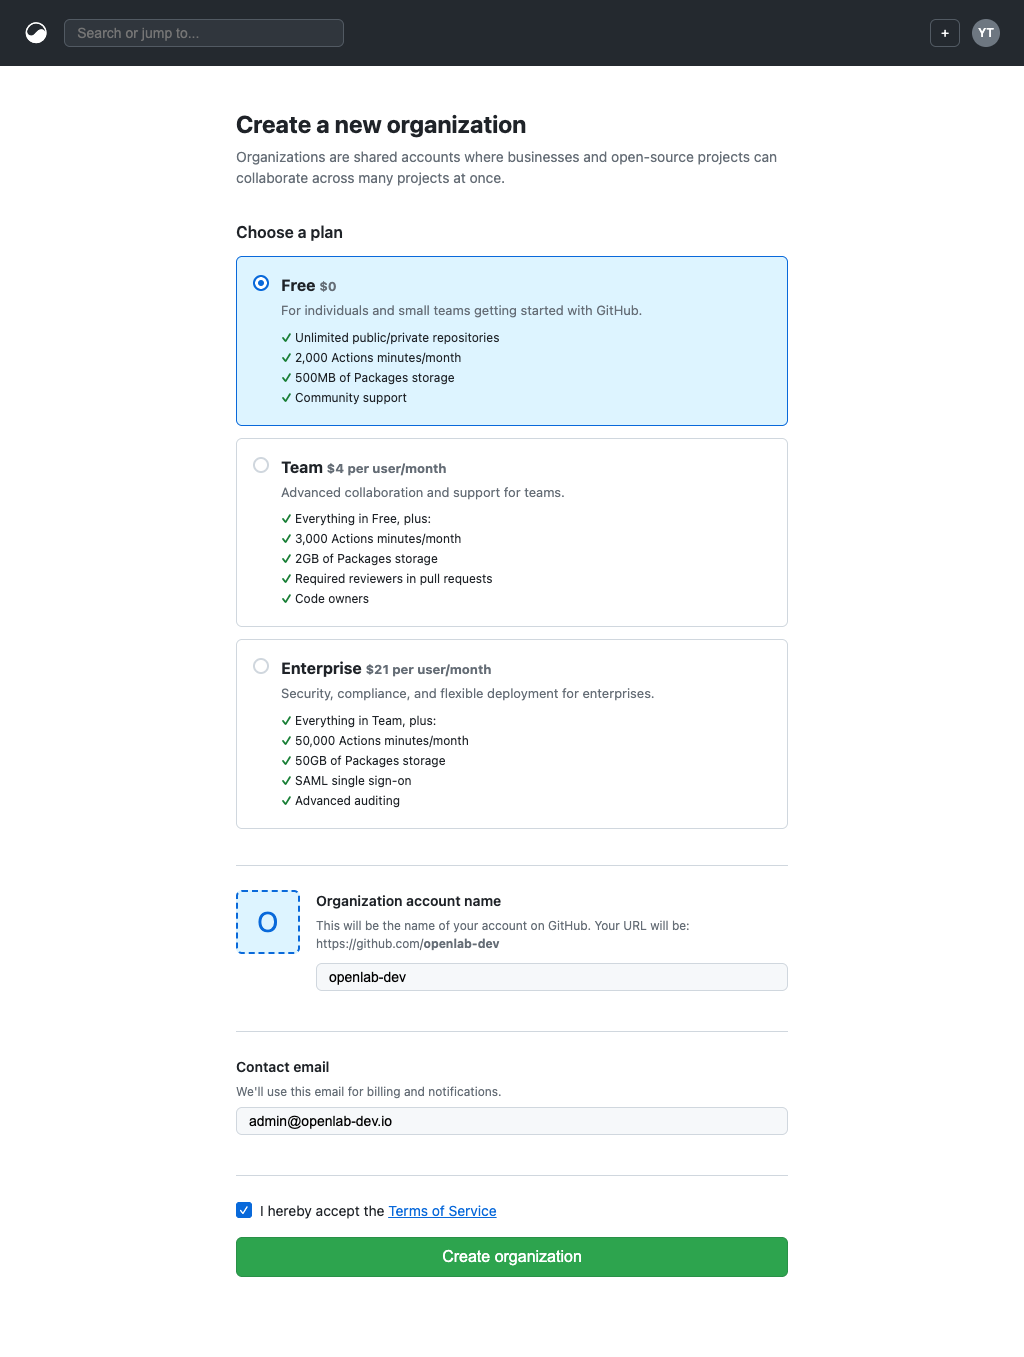
\includegraphics[width=0.95\textwidth]{images/org-create.png}
\caption{Organization作成画面でプランを選択する画面}
\end{figure}

作成が完了したら、CLIから確認してみましょう。

\begin{lstlisting}[language=bash]
# 自分が所属するOrganizationの一覧を表示
gh org list
\end{lstlisting}

Organizationにリポジトリを作成するには、通常のリポジトリ作成と同じコマンドに、Organization名をプレフィックスとして付けます。

\begin{lstlisting}[language=bash]
# Organizationにリポジトリを作成
gh repo create my-org/new-project --public --description "新しいプロジェクト"

# Organizationのリポジトリ一覧を確認
gh repo list my-org
\end{lstlisting}

\section{メンバーの管理}

Organizationにメンバーを追加する際、そのメンバーにどの程度の権限を与えるかを決める必要があります。GitHubのOrganizationには、4つの権限ロールが用意されています。それぞれの役割と責任範囲を正確に理解することが、安全なチーム運営の基礎となります。

\subsection{権限ロールの詳細}

\textbf{Owner（オーナー）}は、Organizationに対する完全な管理権限を持つロールです。Organizationの設定変更、メンバーの追加・削除、リポジトリの作成・削除、請求情報の管理など、すべての操作が可能です。Ownerは最低1人必要ですが、セキュリティの観点から少数に限定することが推奨されます。万が一唯一のOwnerがアカウントにアクセスできなくなった場合に備えて、信頼できるメンバーを2〜3人Ownerに設定しておくとよいでしょう。

\textbf{Member（メンバー）}は、Organizationの一般的なメンバーです。MemberはOrganization自体の設定は変更できませんが、所属するTeamに応じたリポジトリへのアクセス権を持ちます。ほとんどのメンバーはこのロールに設定します。

\textbf{Outside Collaborator（外部コラボレーター）}は、Organization自体には所属せず、特定のリポジトリだけにアクセス権を付与された外部の協力者です。たとえば、業務委託先の開発者や、一時的にプロジェクトに参加するフリーランスのデザイナーなどに適しています。Outside CollaboratorはOrganizationのメンバー一覧には表示されません。

\textbf{Billing Manager（請求管理者）}は、請求情報の閲覧・変更のみが可能な特殊なロールです。経理担当者など、コードにはアクセスする必要がないものの、支払いの管理が必要な人に付与します。

\begin{tabular}{|l|l|l|l|l|l|}
\hline
\textbf{ロール} & \textbf{Org設定} & \textbf{メンバー管理} & \textbf{リポジトリ作成} & \textbf{リポジトリアクセス} & \textbf{請求管理} \\
\hline
\textbf{Owner} & 可能 & 可能 & 可能 & 全リポジトリ & 可能 \\
\hline
\textbf{Member} & 不可 & 不可 & 設定による & Teamに応じる & 不可 \\
\hline
\textbf{Outside Collaborator} & 不可 & 不可 & 不可 & 指定されたリポジトリのみ & 不可 \\
\hline
\textbf{Billing Manager} & 不可 & 不可 & 不可 & なし & 可能 \\
\hline
\end{tabular}

\subsection{メンバーの招待方法}

メンバーの招待は、Web UIから行います。

\begin{enumerate}
  \item Organizationのページを開き、\textbf{People}タブをクリックします
  \item 「\textbf{Invite member}」ボタンをクリックします
  \item 招待したいユーザーのGitHubユーザー名またはメールアドレスを入力します
  \item ロール（Owner または Member）を選択します
  \item 「\textbf{Send invitation}」をクリックします
\end{enumerate}

招待されたユーザーには通知が届き、承認するとOrganizationに参加できます。

\begin{figure}[htbp]
\centering
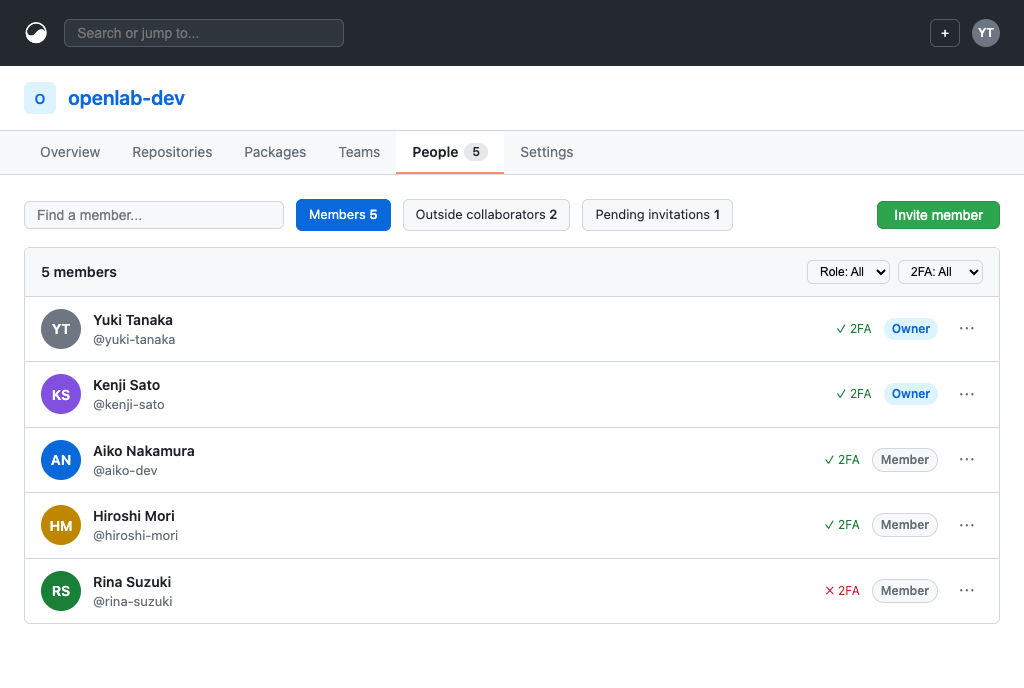
\includegraphics[width=0.95\textwidth]{images/org-members.png}
\caption{メンバー招待画面}
\end{figure}

\section{Teams（チーム）}

Organizationの真価は、Teams機能にあると言っても過言ではありません。Teamsを使うことで、メンバーを論理的なグループに分け、グループ単位でリポジトリへの権限を設定できます。

\subsection{なぜTeamsが必要なのか}

10人のOrganizationに5つのリポジトリがあるとします。Teamsを使わない場合、各メンバーの各リポジトリへの権限を個別に設定する必要があり、最大で50個の権限設定が必要です。メンバーが増えるたびにすべてのリポジトリへの権限を個別に設定しなければなりません。

Teamsを使えば、「frontendチームにはweb-appとdesign-systemリポジトリのWrite権限」のように設定し、新しいフロントエンドエンジニアが入社したら、frontendチームに追加するだけで適切な権限が自動的に付与されます。

\subsection{チームの作成}

チームの作成はWeb UIから行います。

\begin{enumerate}
  \item Organizationのページで\textbf{Teams}タブを開きます
  \item 「\textbf{New team}」ボタンをクリックします
  \item チーム名を入力します（例：\cmd{frontend}、\cmd{backend}、\cmd{devops}）
  \item 説明文を入力します（任意ですが、チームの役割を明記すると分かりやすい）
  \item 可視性を設定します。\textbf{Visible}はOrganizationの全メンバーに公開、\textbf{Secret}はTeamメンバーとOwnerのみに表示されます
  \item メンバーを追加します
\end{enumerate}

\begin{figure}[htbp]
\centering
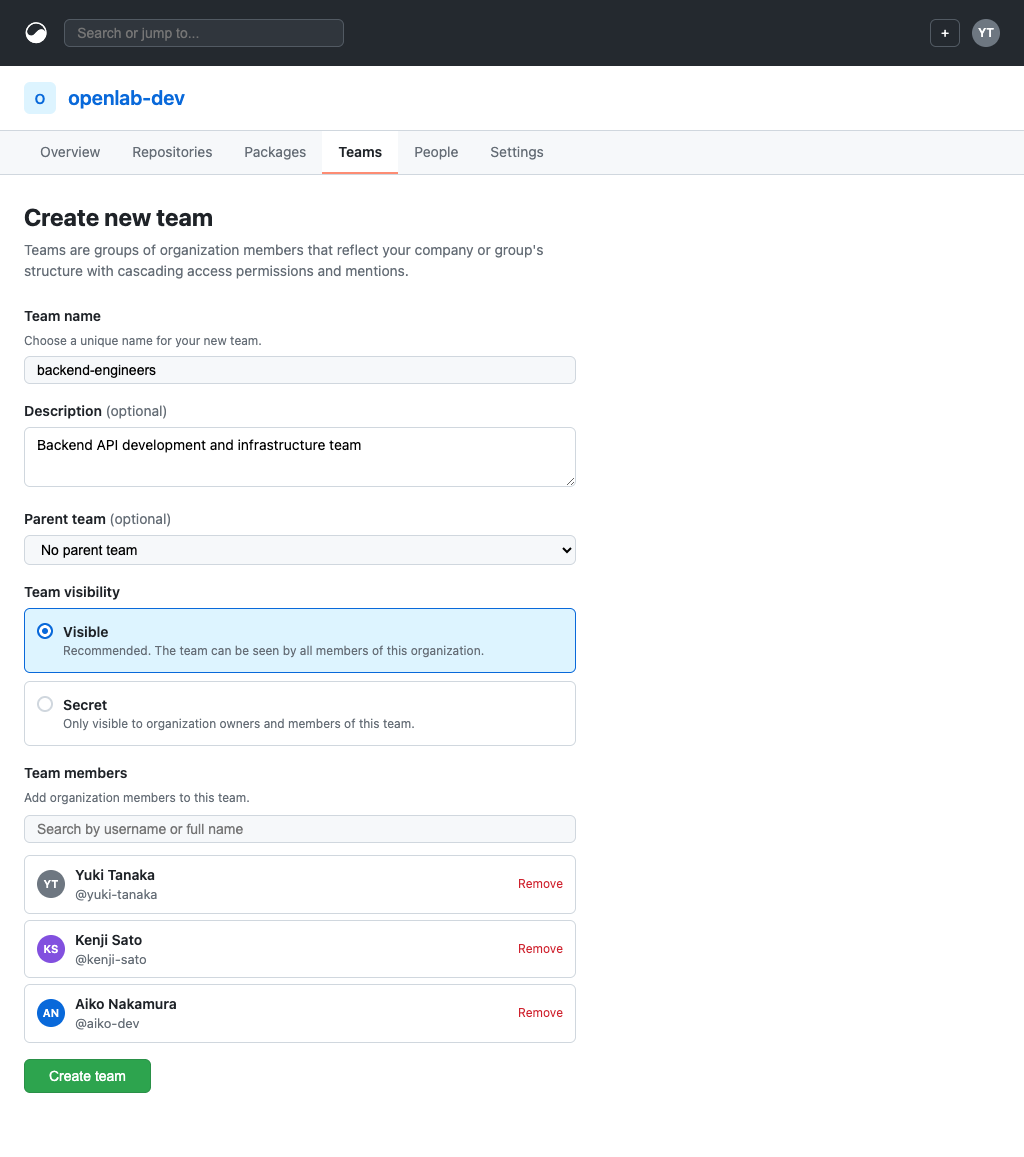
\includegraphics[width=0.95\textwidth]{images/org-team.png}
\caption{チーム作成画面}
\end{figure}

\subsection{チームの権限レベル}

Teamにリポジトリを関連付ける際、5段階の権限レベルから選択できます。権限は低い方から順に、Read、Triage、Write、Maintain、Adminです。上位の権限は下位の権限をすべて含みます。

\textbf{Read（読み取り）}は、リポジトリの閲覧、Issue/PRの閲覧、cloneが可能です。コードを読む必要はあるが、変更は加えないメンバー（PMやデザイナーなど）に適しています。

\textbf{Triage（トリアージ）}は、Readの権限に加えて、Issueやプルリクエストの管理（ラベル付け、アサイン、クローズなど）が可能です。プロジェクトマネージャーやQAエンジニアに適しています。

\textbf{Write（書き込み）}は、リポジトリへのpush、ブランチの作成・削除、PRの作成が可能です。日常的にコードを書く開発者に最も一般的な権限です。

\textbf{Maintain（メンテナンス）}は、Writeの権限に加えて、ブランチ保護ルールの管理やリポジトリの一部設定の変更が可能です。テックリードやシニアエンジニアに適しています。

\textbf{Admin（管理者）}は、リポジトリに対する完全な管理権限です。リポジトリの削除、Webhookの設定、アクセス権の管理などが可能です。

\begin{tabular}{|l|c|c|c|c|c|}
\hline
\textbf{操作} & \textbf{Read} & \textbf{Triage} & \textbf{Write} & \textbf{Maintain} & \textbf{Admin} \\
\hline
コード閲覧・clone & o & o & o & o & o \\
\hline
Issue/PRの管理 & - & o & o & o & o \\
\hline
Push・ブランチ操作 & - & - & o & o & o \\
\hline
ブランチ保護の管理 & - & - & - & o & o \\
\hline
リポジトリ設定変更 & - & - & - & - & o \\
\hline
\end{tabular}

\subsection{ネストされたチーム}

Teamsには\textbf{親子関係（ネスト）}を設定できます。これにより、組織の階層構造をTeamsの構造に反映できます。

\begin{lstlisting}[language={}]
Engineering（親チーム）
├── Frontend（子チーム）
├── Backend（子チーム）
└── DevOps（子チーム）
\end{lstlisting}

子チームは\textbf{親チームの権限を自動的に継承}します。たとえば、EngineeringチームにdocsリポジトリへのRead権限を付与すると、Frontend、Backend、DevOpsの各子チームのメンバーも自動的にdocsリポジトリを閲覧できるようになります。

この仕組みを使えば、全エンジニアに共通する基本権限は親チームで設定し、チーム固有の権限は子チームで追加するという効率的な管理が可能です。

子チームを作成するには、チーム作成時に「Parent team」フィールドで親チームを選択します。

\section{CODEOWNERS}

\subsection{ファイルやディレクトリの担当者を定義する仕組み}

開発チームが大きくなると、「このファイルの変更は誰にレビューしてもらうべきか」という判断が難しくなります。特に、フロントエンドのコード変更をバックエンドエンジニアだけがレビューしてしまったり、重要な設定ファイルの変更がレビューなしでマージされてしまったりすると、問題が発生するリスクがあります。

\textbf{CODEOWNERS}ファイルは、リポジトリ内のファイルやディレクトリごとに「担当者（オーナー）」を定義する仕組みです。CODEOWNERSファイルに記載されたパターンに一致するファイルが変更されたPull Requestが作成されると、対応する担当者が\textbf{自動的にレビュアーとして追加}されます。

CODEOWNERSファイルは、リポジトリのルートディレクトリ、\cmd{docs/}ディレクトリ、または\cmd{.github/}ディレクトリに配置できます。一般的には\cmd{.github/CODEOWNERS}に置かれることが多いです。

\subsection{CODEOWNERSファイルの書き方}

CODEOWNERSファイルの各行は、ファイルパターンとオーナー（ユーザーまたはTeam）の組み合わせで構成されます。パターンの記法は\cmd{.gitignore}と同じglob構文を使います。

\cmd{.github/CODEOWNERS}:
\begin{lstlisting}[language={}]
# デフォルトのオーナー（他のルールに一致しないすべてのファイル）
* @my-org/engineering

# フロントエンドのコード
/src/frontend/          @my-org/frontend
*.tsx                   @my-org/frontend
*.css                   @my-org/frontend

# バックエンドのコード
/src/api/               @my-org/backend
*.py                    @my-org/backend

# データベース関連（特に慎重なレビューが必要）
/migrations/            @my-org/backend @my-org/devops

# ドキュメント
/docs/                  @my-org/docs-team

# CI/CD設定とインフラ
/.github/               @my-org/devops
Dockerfile              @my-org/devops
docker-compose.yml      @my-org/devops

# セキュリティに関わるファイル（Ownerレベルのレビューが必要）
/src/auth/              @security-lead
\end{lstlisting}

いくつかのポイントを補足します。

\textbf{複数のオーナーを指定}できます。\cmd{/migrations/ @my-org/backend @my-org/devops}のように書くと、migrationファイルが変更された場合、backendチームとdevopsチームの両方がレビュアーに追加されます。

\textbf{後の行が優先}されます。同じファイルに複数のパターンが一致する場合、ファイルの後の方に書かれたルールが優先されます。たとえば、最初の行の\cmd{*}は全ファイルに一致しますが、\cmd{/src/frontend/}配下のファイルは後の行のルールで上書きされます。

\textbf{個人とTeamの両方を指定}できます。\cmd{@username}で個人ユーザーを、\cmd{@org-name/team-name}でTeamを指定します。

\subsection{ブランチ保護ルールとの連携}

CODEOWNERSファイルの真価は、ブランチ保護ルールと組み合わせたときに発揮されます。ブランチ保護の設定で「Require review from Code Owners」を有効にすると、CODEOWNERSに定義されたオーナーの承認なしにはPull Requestをマージできなくなります。これにより、重要なファイルの変更が必ず適切な担当者のレビューを経ることが保証されます。

\section{まとめ}

この章では、GitHubのOrganization機能について学びました。重要なポイントを振り返りましょう。

\begin{itemize}
  \item \textbf{Organization}は、チームや企業でリポジトリを共有管理するためのアカウントであり、個人アカウントとは異なる特徴を持つ
  \item Organizationのメンバーには\textbf{Owner、Member、Outside Collaborator、Billing Manager}の4つのロールがあり、それぞれ異なる権限を持つ
  \item \textbf{Teams}を使ってメンバーをグループ化し、Team単位でリポジトリへのアクセス権限（Read〜Admin）を効率的に管理できる
  \item Teamsは\textbf{ネスト（親子関係）}が可能で、子チームは親チームの権限を継承する
  \item \textbf{CODEOWNERS}ファイルを使うことで、ファイルやディレクトリの担当者を定義し、Pull Request作成時に自動的にレビュアーを割り当てることができる
\end{itemize}

Organizationとチーム管理は、プロジェクトの規模が大きくなるにつれてその重要性が増してきます。最初は少人数でも、将来のチーム拡大を見据えて早い段階からOrganizationを導入しておくと、後々の管理がスムーズになります。
